\documentclass[12pt]{report}
\usepackage{algorithmic}
\usepackage{algorithm}
\usepackage{hyperref}
\usepackage{amsmath, amsthm, amssymb}
\usepackage{graphicx}
\newtheorem{mydef}{Definition}
\usepackage{setspace}
\usepackage{ifpdf}
\usepackage{hyperref}
\usepackage{fancyheadings}
\usepackage[a4paper]{geometry}
\geometry{left=1.25 in,top= 1.0in,bottom= 1.0 in,right= 0.75 in}
\doublespacing 
\title{}
\author{}
\date{}
\linespread{2}
\begin{document}
\maketitle
\pagestyle{plain}
\pagenumbering{roman}
\setcounter{page}{6}
\tableofcontents
\newpage
\listoffigures
\newpage


\pagestyle{fancy}
\pagenumbering{arabic}
\fancyhead{}
\fancyfoot{}
\fancyhead[RO,RE]{MRIS approach using LLVM}
\fancyfoot[CO, CE] {\thepage}
\fancyfoot[RO,RE]{Dept of CS \& E, SJCE, Mysore}
\renewcommand{\headrulewidth}{0.4pt}
\renewcommand{\footrulewidth}{0.4pt}

\chapter{Introduction}
\section{Background}
The compiler mainly consists of two phases -- the frontend and the backend. The lexical analysis and the parsing of the source code is done by the frontend of the compiler.  Lexical analysis phase identifies the tokens and builds the symbol table.  The `parser` conforms the source code with the grammar of the language.  It also performs the semantic analysis. Generally, the Intermediate Representation (IR) is generated by the parser of the frontend.

The backend mainly consists of the `code generator`. It takes the intermediate representation as input and maps it into the target language. The target language is the sequence of machine instructions that perform the same task as the input. Reordering of instructions or instruction scheduling \cite{Aho} \cite{Appel} \cite{Muchnick} \cite{Gibbons-Muchnick} and judicious assignment of registers to hold variable values or register allocation \cite{Aho} \cite{Appel} \cite{Muchnick} \cite{Chaitin} \cite{Briggs} are the important phases of code generation. Both instruction scheduling and register allocation tries to reduce the space-time complexity. Backend mainly consists of the `instruction scheduler` and the `register allocator`. It also consists of optimizations that tries to reduce the compile time and execution time. The intermediate representation is handled by the various passes of the backend which finally converts it into the `object` code. Our project concerns with the optimizations in instruction scheduling to reduce execution time.

Figure \ref{fig:com1} shows a very broad overview of compilation stages. Our implementation is at `Basic-block and scheduling 1` of block D.

\begin{figure}[htb]
\begin{center}
\ifpdf
	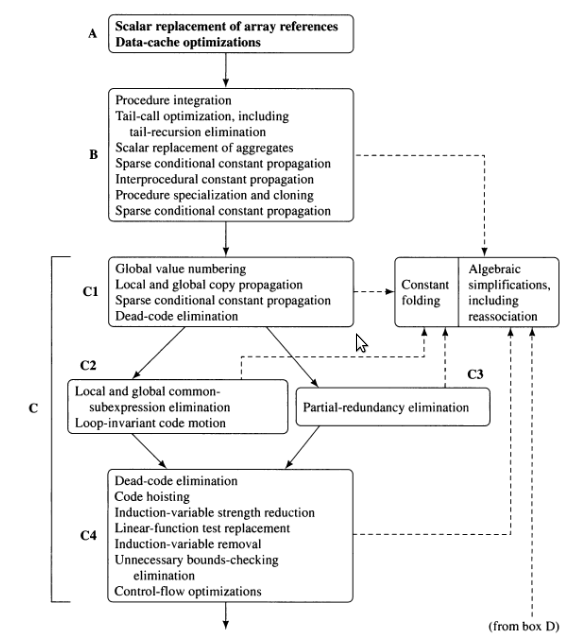
\includegraphics[scale=0.50]{./stage1.png}
\else
\fi
\caption{Compiler stages 1}
\label{fig:com1}
\end{center}
\end{figure}

\begin{figure}[htb]
\begin{center}
\ifpdf
	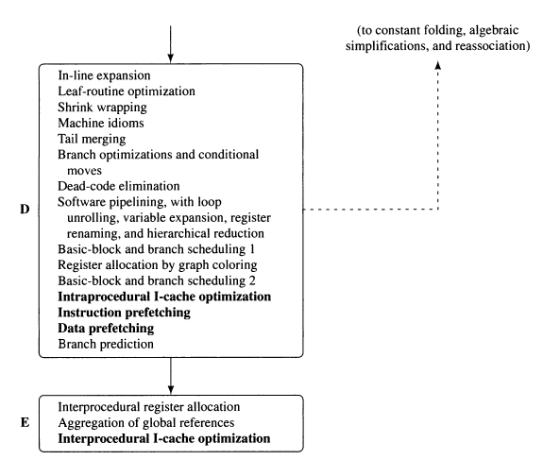
\includegraphics[scale=0.50]{./stage2.png}
\else
\fi
\caption{Compiler stages 2}
\end{center}
\end{figure}

\section{Conventional Scheduling}
A traditional scheduler takes execution latencies of all the instructions in the data dependency graph into account because the main objective is to reduce the length or execution time of the schedule. The list scheduler topologically orders the instructions. Using the order, the instruction is scheduled whose dependencies are satisfied. In case of out-of-order processors, scheduling can be done statically at compile time or dynamically by register renaming. Dynamic scheduling can uncover parallelism obscured by false dependencies. The next section gives a clear overview of scheduling.

\section{Register reduction sequencing}
Decreasing the register pressure decreases spill code \cite{Chaitin} and ultimately decreases the execution time as cited in the next section. In this project, we try to \emph{sequence} the instructions such that they use minimum number of registers and thus decreasing execution time. Our improvement over the conventional scheduling may be stated in the following definition.
\begin{mydef}: {\bf Problem Statement} : Given a data dependence graph G, derive an instruction sequence S for G that is optimal in the sense that its register requirement is minimum.
\end{mydef}


\section{Applications}
\begin{itemize}
\item The Minimum Register Instruction Sequence can be used as an alternative to traditional scheduling in the backend of the compiler. Thus the MRIS can be implemented in all commercial compilers.
\item The MRIS uses less registers during execution reducing the spill code when compared to traditional scheduling. Reduced spilling decreases memory transfers. Thus, an application compiled using the MRIS is likely to consume less power.
\end{itemize}

\chapter{Scheduling concepts and sequencing}
Generally, the instructions are re-ordered by analysing the data dependency graph (DDG) to reduce execution time. But, the number of load and store instructions increases the execution time due to increase in `spill` code. The number of registers are limited in any architecture processor. When the required number of registers are not present to accommodate all the live variables, then some variables are represented in memory and are known as spilled variables. Register pressure is the maximum usage of registers of the processor at any point in the execution sequence of the program. Spilling has more probability with increase in register pressure. Thus if register pressure is reduced, then spilling reduces which ultimately reduces the execution time.

On a processor with instruction-level parallelism, the execution time highly depends on potential parallelism \cite{Architecture} in the program. This program might execute faster if we can \emph{extract} parallelism by reordering instructions from original sequence. Most of the modern processors are out-of-order multiple instruction issue. The processors whose parallelism is managed statically by software are known as Very-Long-Instruction-Word processors and those managed dynamically by hardware are superscalar processors. False dependencies are handled in out-of-order processors by register renaming \cite{Architecture}. It uses the reservation stations to schedule the instructions whose dependencies are satisfied. In this project we are interested in generating an instruction sequence S, statically at compile time, that uses minimum registers and therefore defined as Minimum Register Instruction Sequence (MRIS). In out-of-order processors, spilling decreases parallelism as each load and store reduces the number of dependants and it is a non-trivial operation. Thus reducing spill codes is important:
\begin{itemize}
\item from a performance point of view in architectures that either have a small cache or a large cache miss penalty;
\item from a memory bandwidth usage viewpoint;
\item from an instruction-level parallelism viewpoint as the elimination of some of the spill instructions frees instruction slots to issue other useful instructions;
\item from a power dissipation viewpoint, as load and store instructions contribute to a significant portion of the power consumed;
\item in multi-threaded architectures, minimizing the number of registers in a thread reduces the cost of a thread context switch.
\end{itemize}

Scheduling is a form of program optimization that applies to the machine code produced by code generator. The three constraints for the scheduling are:
\begin{itemize}
\item \emph{Control-dependence constraints}: All the operations executed in the original program must be executed in the optimized one.
\item \emph{Data-dependence constraints}: The operations in the optimized program must produce the same results as the corresponding ones in the original program.
\item \emph{Resource constraints}: The schedule must not oversubscribe the resources on the machine.
\end{itemize}
Scheduling changes the order of instructions and improves execution time. But, the state of the memory at any one point may not match any of the memory states in a sequential execution. This causes debugging problems when the program's execution is interrupted.

\textbf{Data Dependence:} If the execution order of two or more instructions are changed, whose variables are distinct or the instructions read the same variable, then the final result remains the same. But if an instruction writes to a variable read or written by another will result in different values after their order of execution is changed. The relative execution of these instructions must be preserved and such pairs of instructions are \emph{data dependant} \cite{Aho}. The data dependency may be true, anti or output dependant. True dependence exists if a write is followed by a read of the same location, the read depends on the value written. If a read is followed by a write to the same location, then anti-dependence exists. The write does not depend on read but write happens before read, then the read operation picks up a wrong value. Output dependence exists when a write is followed by another write. The memory location will have the value written by the last instruction instead of the exact instruction writing the value. Using different locations to store different values eliminates the dependencies. Figure \ref{fig:DDG} shows the data dependencies between the nodes for the code sequence:\\
c = 1;\\
a = c;\\\\
An edge, known as the dependency edge, from node A to node B indicates that node B is dependant on node A. The graph is known as a data dependency graph, G = (N, E), having a set of N nodes representing the machine instructions' operations and the set of edges E representing the data-dependence constraints among the operations of the instructions. The dashed line indicates the control dependency among the instructions. FrameIndex is a slot used to store the variables. The graph is constructed for each basic block take function unit resource constraints on each operation. In case of traditional scheduling, an edge may be labeled by the latency indicating that the dependant node is to be scheduled after the latency period. The traditional list scheduler topologically orders the nodes of the data-dependency graph. Following the order the instructions are scheduled whose dependencies are satisfied.

\begin{figure}[!h]
\begin{center}
\ifpdf
	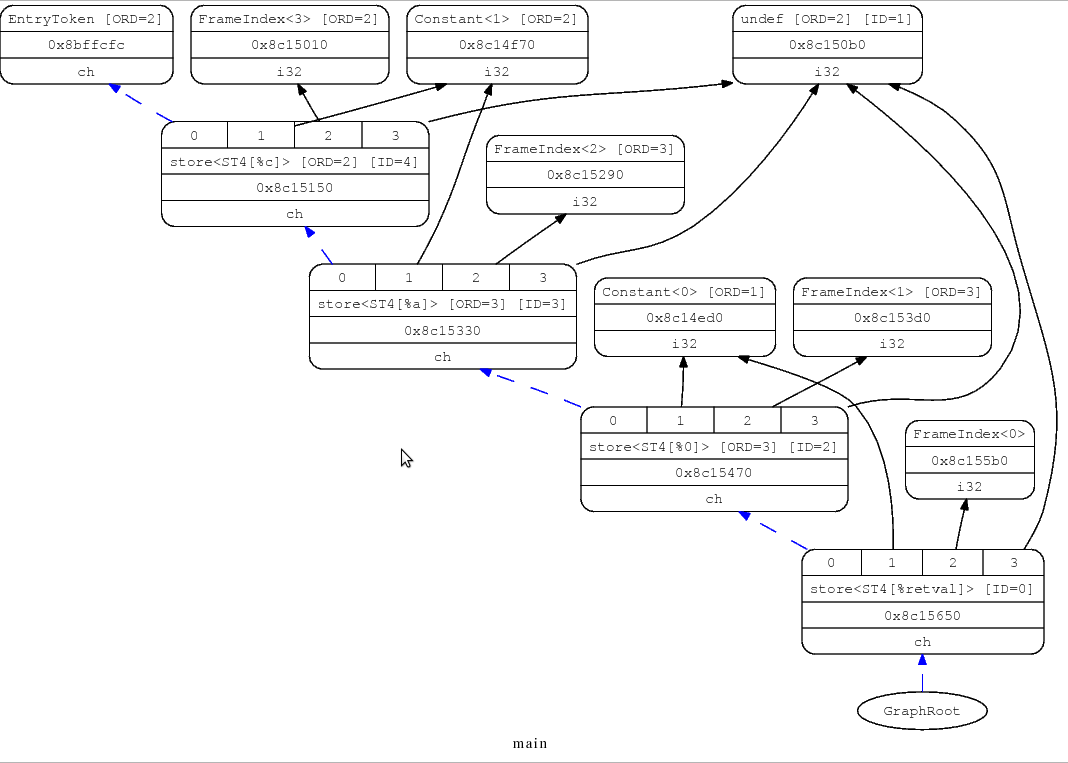
\includegraphics[scale=0.4]{./dataDependence.png}
\else
\fi
\caption{Data-Dependency Graph (DDG)}
\label{fig:DDG}
\end{center}
\end{figure}

The list scheduling algorithm visits the nodes in the chosen prioritized topological order. The instructions are placed in the schedule as early as possible and thus the nodes may get scheduled in approximately the topological order. That is, the list scheduling algorithm computes the earliest time slot in which each node can be executed, according to its data-dependence constraints with the previously scheduled nodes. When all the dependencies are satisfied for a node, it is scheduled. The list scheduling algorithm is shown. It takes the machine resources, R = [r$_1$, r$_2$, ...], where r$_i$ is number of units available of the \emph{i}th kind of resource and the data-dependency graph, G = (N, E). Each operation \emph{n} in N is labeled with its resource-reservation table RT$_n$; each edge e = n$_1$ $\rightarrow$ n$_2$ in E is labeled with d$_e$ indicating that n$_2$ must execute no earlier than d$_e$ clocks after n$_1$. The output is a schedule S that maps the operations in N into time slots in which the operations can be initiated satisfying all the data and resources constraints.
\linespread {1}
\begin{algorithm}
\caption{List\_Scheduling(R, G)}
\begin{algorithmic} [1]
\STATE RT = an empty reservation table;
\FOR {each \emph{n} in N in prioritized topological order}
	\STATE s = max$_{\emph{e}=\emph{p} \rightarrow \emph{n}}$ $_{in}$ $_E$ (S(\emph{p}) + \emph{d}$_\emph{e}$);
	\STATE /* Find the earliest time this instruction could begin, given when its predecessors started. */
	\WHILE {there exists \emph{i} such that RT[\emph{s} + \emph{i}] + RT$_n$[\emph{i}] $>$ R}
	\STATE \emph{s} = \emph{s} + 1;
	\STATE /* Delay the instruction further until the needed resources are available */
	\ENDWHILE
	\STATE S(\emph{n}) = \emph{s};
	\FOR {all \emph{i}}
	\STATE RT[\emph{s} + \emph{i}] = RT[\emph{s} + \emph{i}] + RT[\emph{i}];
	\ENDFOR
\ENDFOR

\end{algorithmic}
\end{algorithm}
\linespread{2}

Sequencing differs by a lot from scheduling. Instruction sequence refers to the arrangement of instructions considering only to reduce the number of registers used or a particular heuristic. The MRIS approach tries to do the same. The input to MRIS problem is a partially ordered small sized data-dependency graph. The partial ordering enables the generation of an instruction sequence that requires less registers. But an instruction scheduler takes into account the latency factors and the availability of function unit resources to arrange the instructions. It also considers true, anti and output dependency constraints whereas the MRIS problem considers only the true dependency constraints. An optimal code generator tries to reduce the schedule length for a fixed number of registers, while the MRIS problem minimizes the number of registers used.

\textbf{Placement of the sequencer:} If registers are allocated before scheduling, the resulting code tends to have many storage dependences that limit code scheduling. On the other hand, if code is scheduled before register allocation, the schedule created may require so many registers that register spilling will negate the advantages of instruction-level parallelism. Thus the ordering between scheduling and register allocation determines the resultant code. Generally, the scheduler is run both before and after the register allocation. The minimum register instruction sequencer tries to reduce the number of registers. Thus, it would be better to sequence the instructions first and pass them to the register allocator because it is more likely for the register allocator to allocate minimum registers for the sequence. Finally, the post-register allocation is performed.

The proposed MRIS method tries to build instruction lineages which are chain of instructions that use the same register. The lineages are fused, that is, two or more lineages which can use the same register are combined. This reduces parallelism and it is a trade off with usage of less registers to improve execution time. When two or more lineages need to run in parallel, they are represented by an interference edge in the lineage interference graph. This graph is colored by any of the graph coloring algorithms and a virtual register is allocated to each instruction of the entire lineage. Logically this method decreases the number of loads and stores and should improve the execution time.

\chapter{MRIS- The approach}
For an Out-Of-Order issue processor which has many execution units, the ability to execute more than one instructions at the same time increases the yield for the program.  But the problem of finding those instructions which can execute parallelly is difficult.  Instructions have data dependencies on other instructions.  That means, an Instruction makes use of the result produced by some other Instruction.  An Instruction cannot start execution until all its Data Dependencies are satisfied.  To make use of the ability of the OOO processor \cite{Architecture}, Instructions which have all there Data Dependencies satisfied at that particular point need to be executed parallelly.  The Scheduling \cite{Muchnick} \cite{Gibbons-Muchnick} phase re-orders the Instructions such that number of cycles the program has to wait for dependencies to satisfy is reduced thus reducing the execution time.  It takes in account the Latency of each of the Instruction before finding a schedule.  The variables that are represented in each instructions are to given register to store their values. Since the target processor has limited number of registers, the compiler will encompass a separate phase of Register allocation where each of the variables described in the aforementioned instructions will be mapped to a physical register. If two variables are needed at a same point, those values need to represented in two different registers. If the program has many such variables, the need for more registers also increases.  But since the number of registers are limited in any architecture processor, some variable of the program will have to be represented in memory rather than registers.  This is called spilling \cite{Chaitin}. Spilling leads to the introduction of Loads and Stores for the variables which are spilled. This make the program to have more Storage dependencies (Anti-dependencies). For an Out-of-order(OOO) processor this means that is takes longer time resolving the dependencies because Load and store instructions takes longer time to execute. This hits hard on the performance of OOO processors. 

The Minimum Register Instruction Sequencing (MRIS) \cite{R. Govindarajan et al.} tries to reduce the Register pressure of the program by rearranging the instructions.  The solution tries to find a set of instructions that can definitely share a register.  This set of Instructions is defined as a \emph{Lineage}.  A single register is allocated to each of the lineages and all the instructions in a lineage will use the same register to produce their result.  The lineages are constructed to have as many instructions in them as possible.  Thus, allocating a single register to many instructions reduces the Register Pressure on the program.  

\section{Motivating Example}
The live range of a variable starts at the point of definition of that variable and ends at the last use.  If two variables are simultaneously live at any point in the program, then those two variable need separate registers to store there values.  These live ranges interfere with one another.  The interfering live variables increases the register pressure since each of the live variables have to be represented by a separate register.  The Non-interfering live variables can use a same register, thereby decreasing the register pressure of the program.

The Data Dependency Graph (DDG) represents the dependencies of instructions on one another.  The nodes represents the Instructions while an edge tells about the data flow from one instruction to another.  DDG can be called as the Data flow of the program.  Any sequence of instructions that will be generated has to conform to the DDG.  An example DDG is shown in the figure \ref{fig:1}.

\linespread{1}
\begin{figure}[htb]
\begin{center}
\ifpdf
	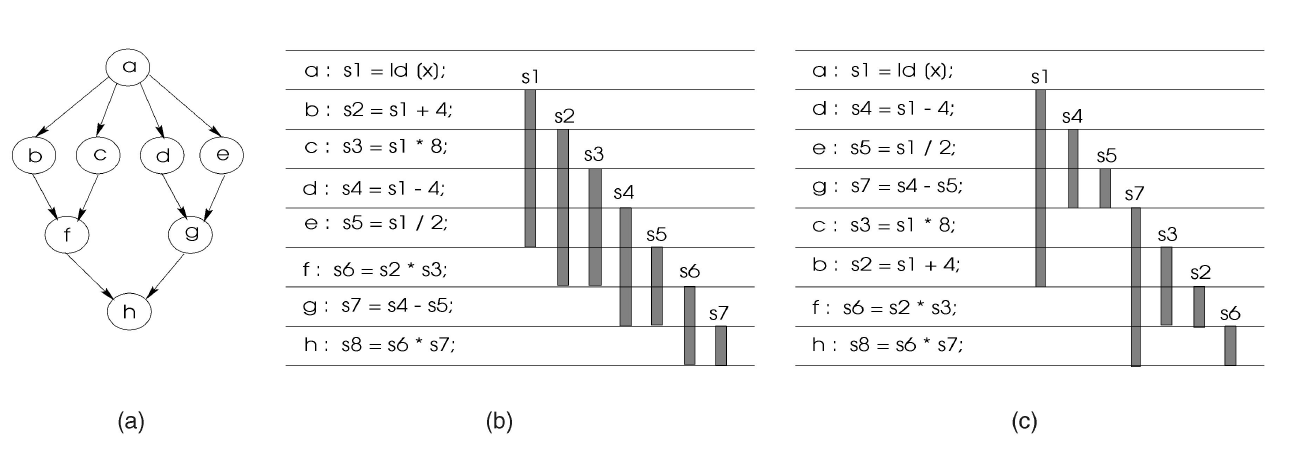
\includegraphics[scale=0.45]{sequence.png}
\else
%	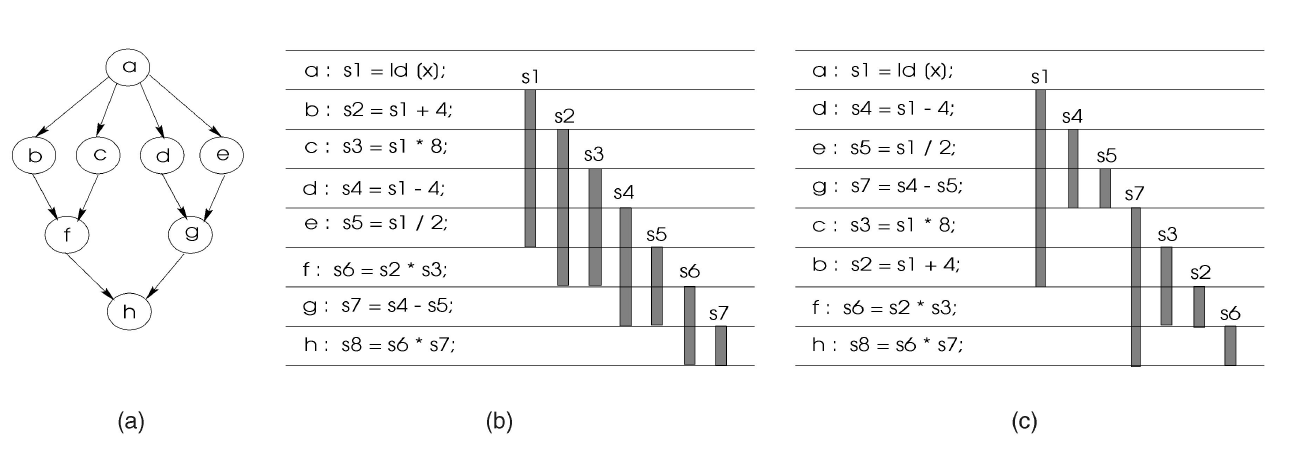
\includegraphics[scale=0.45]{sequence.png}
\fi
\caption[A motivating example of sequencing]{An example. (a)DDG. (b) Instruction Sequence 1. (c) Instruction Sequence 2}
\label{fig:1}
\end{center}
\end{figure}
\linespread{2}

The figure \ref{fig:1} gives a Data dependency graph and two of the possible instruction sequence. Both of the Instruction sequences conform to the given DDG.  Also the live ranges of each of the variables produced by the instruction is given.  The number of overlapping live ranges in the instruction sequence 1 is 4 and its 3 for the instruction sequence 2.  Comparing both the instruction sequence, the sequence 2 has minimum register pressure than that of sequence 1.  In the DDG, the node \emph b passes the value that it produced to node \emph f and since there is no other nodes that uses the value of \emph b, we can definitely say that in any instruction sequence, the register that is assigned to \emph b can be reused by \emph f.  Similarly the nodes \emph e and \emph g can share the same register.  Now, can \emph f and \emph g share the same register? No. Because both the instructions produce values that is used by the node \emph h.  Hence nodes \emph f and \emph g interfere in all the possible instruction sequence and need separate registers for each one of them.  Now considering the nodes \emph c and \emph d, although both are interfering in the instruction sequence 1, the sequence 2 places \emph c and \emph d such that they are not live simultaneously.  This makes the nodes \emph c and \emph d share a same register.  The DDG tells about the nodes that definitely overlap and those that may not overlap for all the instruction sequence.  In order a generate a minimal register pressure instruction sequence, the nodes that can definitely share a register has to be identified.

The MRIS approach is bounded by the concept of \emph{Lineages}. Lineage is a set of Instructions that can definitely share a register.  The instructions for a Lineage are selected based on the DDG.  A node will pass on its value to its descendant.  If there are multiple descendants then one of them is chosen to be the heir.  Hence the register that is used by the parent to store its value will be passed on to its heir.  Such sequence of instructions I$_1$, I$_2$, I$_3$... I$_n$ where I$_2$ is a heir of I$_1$, I$_3$ as heir of I$_2$ and so on, will form an Instruction Lineage.  All the instructions in a lineage will share a same register, as the register is passed onto from one instruction to another.  

Since the Instruction sequence that will be generated must conform to the DDG, the instructions in a lineage has a implicit order of execution.  The heir of a node cannot execute until its parent finishes its execution.  If a parent has many descendants, the heir of the parent node must not start execution until all other descendants of the parent node finishes use of the value produced by the parent. Hence the order of execution should have parent node and all the descendants of the parent node other than the heir and then only the heir of the parent node starts execution.  This sequencing constraint is represented by having an \emph{Sequencing edges} from other descendants of the parent node to its heir.  This results in the updating of the DDG called the \emph{Augmented DDG}.  The original DDG and its corresponding Augmented DDG is represented in the Figure \ref{fig:2}.

\linespread{1}
\begin{figure}[htb]
\begin{center}
\ifpdf
	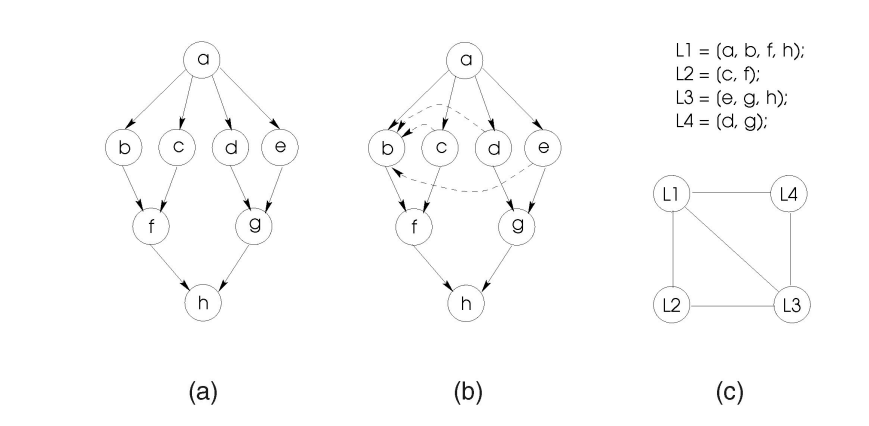
\includegraphics[scale=0.50]{lig.png}
\else
%	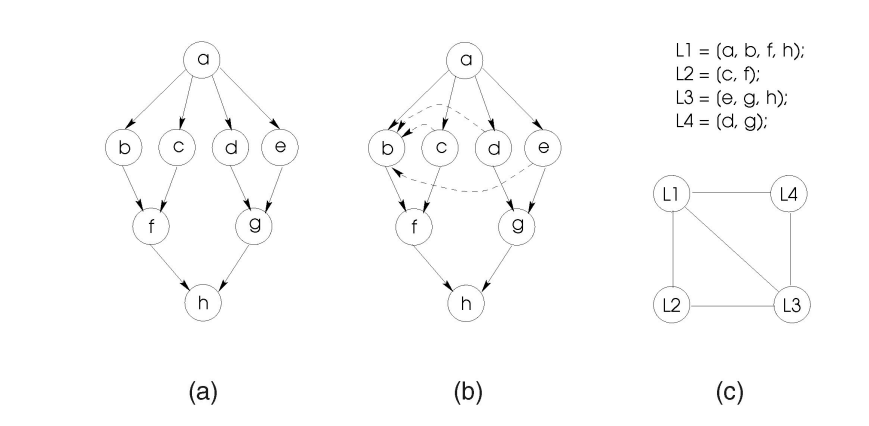
\includegraphics[scale=0.50]{lig.png}
\fi
\caption[Data dependence graph for the motivating example]{Data dependence graph for the motivating example. (a) Original DDG. (b) Augmented DDG. (c) Lineage interference graph.}
\label{fig:2}
\end{center}
\end{figure}
\linespread{2}

For the given DDG, the lineages are 

\hspace{1in}L$_1$ = \{a, b, f, h\}

\hspace{1in}L$_2$ = \{c, f\}

\hspace{1in}L$_3$ = \{e, g, h\}

\hspace{1in}L$_4$ = \{d, g\}

The lineage start from the point where the first instruction produces the value in a register and ends at the last use of that register for that lineage.  Hence the lineages are represented as the def-last\_use relation of instructions wherein the last instruction uses the value in the register.  The last instruction may be part of another lineage.  Thus we represent this relation starting with a closed interval and ending the lineage by a open interval.  This representation for the lineages generated above will be,

\hspace{1in}L$_1$ = [a, b, f, h)

\hspace{1in}L$_2$ = [c, f)

\hspace{1in}L$_3$ = [e, g, h)

\hspace{1in}L$_4$ = [d, g)

After having defined the set the instructions that can definitely share a register as lineages, the process of Register Allocation of instruction in the program is now to allocate registers for the lineages.  The live range of a lineage is the concatenation of the live ranges of the instructions that the lineage contain.  To determine the interference between two lineages, we have to see whether the live range of the two lineages overlap in all legal sequence of instructions.  If the live range of two lineages overlap in all the instruction sequences then they cannot share a register.  This is represented by having an edge between the two lineages in the Lineage Interference Graph(LIG).  If two lineages does not overlap at least in some legal instruction sequences, then the two lineages can share a same register given that there is some ordering of instructions between the lineages.  The Lineage Interference Graph is constructed by the data of the lineages interfering with each other.  The traditional coloring approach \cite{Chaitin} \cite{Briggs} is used to color the LIR.  The minimum number of color required to color the LIR give the minimum number of register needed for executing the program.  This number is called the Heuristic Register Bound(HRB).

The sequencing of the instructions is done using the coloring of lineages and the DDG of the program so that the sequence generated has minimum register pressure.  

\section{Lineage Formation}
A node may have many immediate descendants in a DDG, but there can only be one node among them that can be selected as the heir. An heir inherits the register form its parent node and hence becomes a part of the lineage. This imposes a restriction that the heir must be the last one among the descendants of the node to be executed as it redefines the register shared by the parent and the value is lost after redefinition.\\

The lineage formation algorithm attempt to form as long lineages as possible. The heir in any lineage is the last one to be executed, hence the live ranges of the instructions do not interfere with each other and all the instructions in the lineage can share the same register. In order to ensure that the heir is the last one to be executed, the algorithm introduces \emph{sequencing edges}. A sequencing edge from node \emph{$v_{i}$} to \emph{$v_{j}$} imposes the constraint that \emph{$v_{i}$} must be listed before \emph{$v_{j}$}. This implies that all the nodes that reach \emph{$v_{i}$} must be listed before any node from \emph{$v_{j}$} is listed. The algorithm makes sure that the introduction of sequencing edges does not make the graph cyclic, which would make it impossible to obtain a sequence for the instructions in the DDG, by using the \emph{height} property to select the heir. The \emph{height} of a node is computed as per the equation
\vspace{24pt}
\begin{equation*}
ht(u) =
\begin{cases}
1 & \text{if \emph{u} has no descendants }\\
1 + max_{\emph{v}\epsilon\emph{D(u)}} \emph{(ht(v))} & \text{otherwise,}\\
\end{cases}
\end{equation*}
\vspace{24pt}

During the lineage formation, if a node \emph{$v_{i}$} has multiple descendants, then the algorithm chooses the node which is having the lowest height among the descendants to be the heir of \emph{$v_{i}$}. If two or more nodes have the same height then the algorithm arbitrarily breaks the tie and it recomputes the height of each node after the introduction of sequencing edges to avoid the formation of cycles. Lineages are formed by the arcs between the nodes and the chosen heirs. Each arc that is a part of a lineage is the def-last-use arc in DDG. \\

The Lineage Formation algorithm is essentially a greedy depth first graph traversal algorithm which identifies the heir of each node by the height property. The algorithm introduces sequencing edges after the heir of a node is selected if the node has multiple descendants and the heights of all the nodes in the DDG are recomputed. The algorithm distinguishes between the sequencing edges and the flow edges. If there is a sequencing edge between node \emph{$v_{i}$} to node \emph{$v_{j}$}, then \emph{$v_{j}$} is not considered as the descendant of \emph{$v_{i}$} for the purpose of lineage formation. Only those arcs that represent data dependences are considered for lineage formation. \\
\linespread {1}
\begin{algorithm}
\caption{Lineage\_Formation(V, E)}
\begin{algorithmic} [1]
\STATE mark all nodes in DDG as \emph{not in any lineage}
\STATE compute the height of every node in DDG
\WHILE { there is a node \emph{not in any lineage} }
	\STATE  recompute height $\leftarrow false $
	\STATE \emph{$v_i$} $\leftarrow$ highest node not in lineage
	\STATE start a new lineage containing \emph{$v_i$}
	\STATE mark \emph{$v_i$} as \emph{in a lineage}
	\WHILE { \emph{$v_i$} has a descendant }
		\STATE \emph{$v_j$} $\leftarrow$ lowest descendant of \emph{$v_i$}
		\IF { \emph{$v_i$} has multiple descendants}
			\STATE recompute height $\leftarrow$ true
			\FOR { each descendant \emph{$v_k$} $\neq$ \emph{$v_j$} of \emph{$v_i$} }
				\STATE add sequencing edge from \emph{$v_k$} to \emph{$v_j$}
			\ENDFOR
		\ENDIF
		\STATE add \emph{$v_j$} to lineage
		\IF {\emph{$v_j$} is already marked as \emph{in a lineage} }
			\STATE end lineage with \emph{$v_j$} as the last node
			\STATE \textbf{break} ;
		\ENDIF
		\STATE mark \emph{$v_j$} as \emph{in lineage}
		\STATE \emph{$v_i$} $\leftarrow$ \emph{$v_j$}
	\ENDWHILE
	\IF { recompute height = true}
		\STATE recompute the height of every node in the DDG
	\ENDIF
\ENDWHILE
\end{algorithmic}
\end{algorithm}
\linespread{2}
\section{Lineage Interference Graph}
By determining the live ranges of two lineages and verifying that the two lineages do not overlap, it is possible to make the two lineages share the same register. The live range of a register is given by the definition-

\begin{mydef}
 If $v_1$, the first instruction of a lineage $L = [ v_1,v_2,....,v_n)$ is in position $t_i$, and the last instruction $v_n$ of L is in the position $t_j$ in an instruction sequence , then the \textbf{live range} of the lineage L starts at $t_{i+1}$ and ends at $t_j$.
\end{mydef}

The live range of a lineage is always contiguous, irrespective of interleaving of instructions from multiple lineages. Thus the live range is active from the listing of the first instruction in the lineage until the listing of the last instruction. \\

In order to determine whether the live ranges of two lineages must necessarily overlap, a condition is defined based on the existence of paths between the lineages. Two sets of nodes are defined. S is the set of nodes that start lineages and E is the set of nodes that end lineages. Then a \emph{reach} relation R is defined as \\

\begin{mydef}
The reach relation R: S $\rightarrow$ E maps S to E. For all $v_a$ $\in$ S and $v_b$ $\in$ E, node $v_a$ reaches node $v_b$ , $R(v_a, v_b) = 1$, if there is a path in the augmented DDG from $v_a$ to $v_b$. Otherwise, $R(v_a, v_b) = 0$.\\
\end{mydef}

The reach relation is used to determine whether the live ranges of two lineages must necessarily overlap in all legal instruction sequences for the augmented DDG.

\begin{mydef}
Two lineages, $L_{u} = [u_{1},u_{2},....,u_{m})$ and $L_{v} = [v_{1}, v_{2},...., v_{n})$, \textbf{definitely overlap} if they overlap in all possible instruction sequences. \\
\end{mydef}

The Lineage Interference Graph (LIG) is constructed as an undirected graph whose nodes represent lineages. The graph contains a arc between two nodes if and only if the live ranges of lineages represented by the nodes \emph{definitely overlap}. Essentially there is a edge in LIG between two lineages $L_{u} = [u_{1},u_{2},....,u_{m})$ and $L_{v} = [v_{1}, v_{2},...., v_{n})$ if and only if $\emph{R($u_{1}$,$v_{n}$)} = 1$ and $\emph{$R(v_{1}$,$u_{m}$)} = 1$. \\

\section{Lineage Fusion}
Let there be two lineages $L_{u} = [u_{1},u_{2},....,u_{m})$ and $L_{v} = [v_{1}, v_{2},...., v_{n})$. The two lineages do not necessarily overlap if $\emph{R($u_{1}$,$v_{n}$)} = 1$ and $\emph{$R(v_{1}$,$u_{m}$)} = 0$, i.e $u_{1}$ reaches $v_n$ , but $v_1$ does not reach $u_m$. Therefore there is always a possibility to find a legal sequence where the two live ranges do not overlap, and both lineages can share the same register. Conversely if the nodes of $L_v$ are listed in the instruction sequence before all the nodes in $L_u$ are listed; the two lineages interfere and cannot share the same register.\\

This can be prevented by introducing new sequencing constraint in DDG. The constraint forces all the nodes of $L_u$ to be listed before any node of $L_v$ is listed. This is called \emph{lineage fusion}. As the name suggests, the lineage fusion operation fuses two lineages which may not necessarily interfere into a single lineage and treat the two lineages $L_u$ and $L_v$ as if they are a single lineage. Lineage fusion also reduces the number of nodes in the lineage interference graph, there by reducing the cost of coloring the graph. Formally Lineage Fusion is defined as\\

\begin{mydef}
Two lineages $L_u$ = [$u_1$, $u_2$,....,$u_m$) and $L_v$ = [$v_1$, $v_2$,...., $v_n$) can be fused into a single lineage if:
	\begin{itemize}
	\item $u_1$ reaches $v_n$, i.e., $R(u_{1}, v_{n}) = 1$;
	\item $v_1$ does not reach $u_m$, i.e., $R(v_{1}, u_{m}) = 0$.\\
	\end{itemize}
\end{mydef}

When the lineages $L_u$ and $L_v$ are fused together, a sequencing edge from $u_m$ to $v_1$ is inserted in the DDG. The lineages $L_u$ and $L_v$ are removed and a new lineage $L_{w} = [u_{1}, u_{2},...., u_{m}) \cup [v_{1}, v_{2},...., v_{n})$ is inserted in the lineage set. The last node of the first lineage, $u_m$ , does not necessarily use the same registers as the other nodes in the new $L_w$ lineage. Thus, it is important to represent the lineage resulting from the fusion as a union of semi-open sequences. \\

Fusing two lineages causes the corresponding nodes in the interference graph to be combined into a single node, say \emph{w}. Every edge that was incident on the either of the nodes in the lineages before fusing is now incident on \emph{w}. As a consequence, the interference graph is updated after each such fusion operation. It is also legal to fuse lineages which are completely independent, i.e. when $R(u_{1}, v_{n}) = 0$ and $R(v_{1}, u_{m}) = 0$. However such fusions would impose unnecessary constraints in the sequencing of $L_u$ and $L_v$. The coloring algorithm indicates such situations thus providing freedom for sequencing algorithm.\\

Lineage fusion is applied after the lineage formation and before the coloring of the lineage interference graph. The reason being that the interference graph to be colored would have less number of nodes and would require less number of colors.\\

To find the lineages that can be fused, the set of lineages is searched for $L_u$ = [$u_1$, $u_2$,....,$u_m$) and $L_v$ = [$v_1$, $v_2$,...., $v_n$) such that $R(u_{1}, v_{n}) = 1$ and $R(v_{1}, u_{m}) = 0$. In accordance to the fusion condition a new lineage is formed as $L_w$ = $L_u$ $\cup$ $L_v$, which requires that a new sequencing edge must be added from $u_m$ to $v_1$. The addition of this new edge necessitates the updating of reach relation. The algorithm updates the reach relation such that all the nodes that could reach $u_m$ prior to the fusion can also reach $v_n$ after the fusion. Now $v_1$ is no longer the start node of the fused lineage $L_w$, and hence the row corresponding to node $v_1$ is discarded from the reach relation. Similarly, if $u_m$ does not terminate any other lineage, its column can also be discarded from the reach relation. Further $v_1$ is removed from the set start nodes S, and $u_m$ is removed from the set of end nodes E, if $u_m$ does not end any other lineages other than $L_w$.\\

If there are multiple candidates for lineage fusion, the algorithm arbitrarily selects two lineages and performs the fusion operation. Each fusion results in the updating of sets S, E and reach relation R. The algorithm continues to search for a suitable pair to fuse until it finds none. It is also possible that a fused lineage $L_u$ $\cup$ $L_v$ may again be fused with some other lineage, say $L_x$ (if they form a legal pair to fuse), thus resulting in a compound lineage $L_u$ $\cup$ $L_v$ $\cup$ $L_x$. The order in which the lineages are fused will determine the size of the interference graph and hence the heuristic register bound values. Different order in the fusion of lineages produces different heuristic register bound values.\\

\section{Coloring the Interference Graph}

The Lineage Interference Graph can be colored using a heuristic graph coloring algorithm \cite{Chaitin} \cite{Briggs}. The number of colors required to color the interference graph is referred to as the Heuristic Register Bound (HRB). Due to the heuristics involved in coloring and due to the sequencing order of descendants nodes in DDG, the HRB computed is near-optimal solution and graph coloring generally is NP-complete \cite{Cormen}.\\

\section{Instruction Sequence Generation}

Once the coloring of the Lineage Interference Graph is completed, each lineage is associated with a register and hence the nodes in the lineage. It is assumed that those registers that are live-in and live-out in the DDG are assigned by the Global Register Allocator. This implementation accounts for the live-in and live-out of registers by the dummy \emph{source} and \emph{sink} nodes.\\

The sequencing algorithm used here is a modified list scheduling algorithm. It uses the information obtained from the coloring of the interference graph, and \emph{lists} the nodes from a ready list based on the height priority and availability of registers assigned to them.\\

\linespread {1}
\begin{algorithm}
\caption{Sequencing($G^|$, L, A)}
\begin{algorithmic} [1]
\STATE ReadyList $\leftarrow$ \{($v_i$, $R_j$) such that $v_i$ has no predecessor \}
\STATE RegAvailable $\leftarrow$ \{$R_1$, $R_2$,....,$R_N$\}
\WHILE { ReadyList $\neq$ $\phi$ }
	\FOR {each node $v_i$ in the ReadyList in decreasing height order}
		\IF {($v_i$ $\notin$ S) \textbf{or} ((($v_i$, $R_j$) $\in$ A) \textbf{and} ($R_j$ $\in$ RegAvailable)) }
			\STATE // either $v_i$ is not n start node of lineage or
			\STATE // the register assigned to $v_i$ in A is available
			\STATE Remove $R_j$ from RegAvailable
			\STATE Remove ($v_i$, $R_j$) from ReadyLIst
			\STATE List ($v_i$, $R_j$)
			\STATE Add to the ready list all successors of $v-i$ that have a;; its predecessor listed
			\IF {($v_i$ $\in$ E) \textbf{and} ($v_i$, $R_j$) $\in$ A}
				\STATE // node $v-i$ ends a lineage which
				\STATE// is assigned register $R_j$
				\STATE Return $R_j$ to RegAvailable
			\ENDIF
		\ENDIF	
	\ENDFOR
\ENDWHILE
\end{algorithmic}
\end{algorithm}
\linespread{2}

The sequencing algorithm takes inputs $G^|$, the augmented DDG with sequencing edges, \emph{L}, list of lineages obtained from the lineage formation algorithm and after the lineage fusion is applied, and \emph{A}, the register assignment for the nodes from the coloring of the lineage interference graph.\\

This algorithm may result in a deadlock due to two reasons. First, the order of listing of nodes belonging to two different lineages having the same color assigned may result in deadlock. Such type of deadlocks are referred to as \emph{avoidable deadlocks}. These can be avoided by applying the lineage fusion. The other kind of deadlocks, referred to as \emph{unavoidable deadlocks}, arise due to the underestimation of HRB. This could happen because the condition used to test if two live ranges definitely overlap is sufficient but not necessary.\\

\linespread{1}
\begin{figure}[htb]
\begin{center}
\ifpdf
	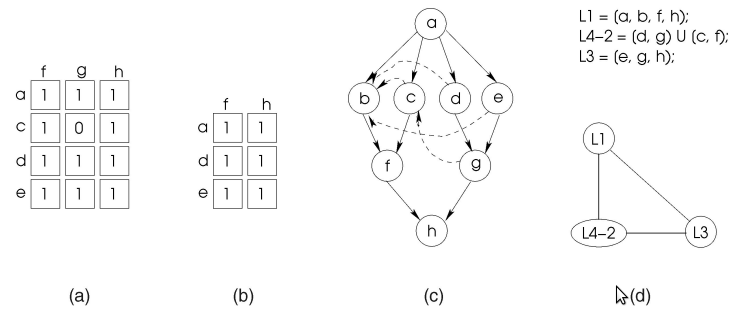
\includegraphics[scale=0.45]{final_sequence.png}
\else
%	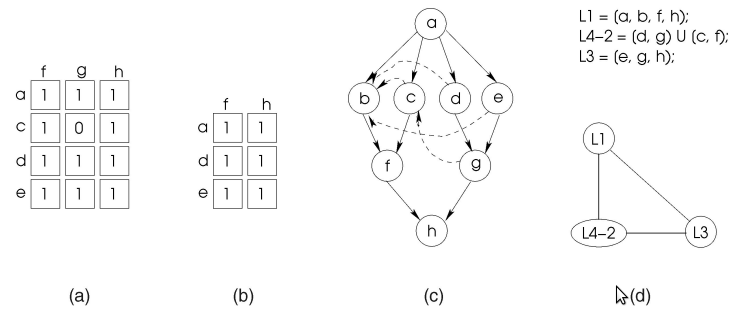
\includegraphics[scale=0.45]{final_sequence.png}
\fi
\caption[Reach relation, DDG and LIG after lineage fusion for motivating example]{Reach relation. DDG and LIG after lineage fusion for motivating example. (a) Reachability before fusion. (b) Reachability after fusion. (c) DDG after fusion. (d) LIG after lineage fusion. }
\label{fig:reach}
\end{center}
\end{figure}
\linespread{2}
When the sequencing algorithm is applied to the motivating example, first the node \emph{a} is listed. Then among the descendants of \emph{a}, node \emph{b} is already chosen to be the heir of node \emph{a} as it is the part of the same lineage. If lineage fusion is not used, listing of \emph{a} causes nodes \emph{c, d, e} to be added to Ready List. The next node that can be listed is node \emph{e} as it is under a separate lineage, \emph{$L_3$}, and register \emph{$R_3$} is available. Now the sequencing algorithm is left with only one register \emph{$R_2$} and either of node \emph{d} or \emph{c} can be listed next. The algorithm breaks the tie arbitrarily and chooses one among the remaining two nodes. If it chooses node \emph{c} to be listed next, an unnecessary cycle of dependencies is created. Node \emph{d} cannot be listed until node \emph{f} is listed, which would then release register \emph{$R_2$}. But to list node \emph{f}, node \emph{b} has to be listed first. Since node \emph{b} must be the last use of of \emph{$R_1$}, it cannot be listed before node \emph{d}. This creates cyclic dependencies and the sequencing algorithm deadlocks. However, this type of deadlock is avoidable deadlock and can be prevented by the process of lineage fusion. When lineage fusion is applied to above case, lineages \emph{$L_2$} and \emph{$L_4$} are fused together and a sequencing edge from node \emph{g} to node \emph{c} is added to the graph, which ensures that node \emph{d} is listed before node \emph{c}. The sequencing algorithm then lists nodes \emph{d, g, c, b, f} and \emph{h} in order thereby using only three registers as predicted by the coloring algorithm.\\

Even with the application of lineage fusion, unavoidable deadlocks occur when the HRB computed by the register coloring algorithm is lower than the number of registers actually needed. In such cases there does not exist a legal sequence of instructions that uses HRB or lower number of registers. The simple approach to overcome this is to increase the HRB value computed by one. The algorithm then picks up one node in the Ready List and changes it register assignment to a new register ( and for the remaining nodes as well). This strategy overcomes the deadlock by gradually increasing the HRB value and trying to obtain a legal sequence of instructions with as few extra register as possible.\\

\chapter{Implementation}
The sequencing by MRIS approach is implemented in the Low-Level Virtual Machine (LLVM) Compiler Infrastructure \cite{LLVM}.  LLVM is purely an object oriented infrastructure implemented in C++. LLVM-GCC is a LLVM C front end which converts the source code to object form. The backend of LLVM converts this object code to executable.  This backend has the capability to perform various optimizations. The best thing about using LLVM is that every stage of the compiler is separated distinctly with different passes, handled by the pass-manager, for each stage. A pass can be disabled deliberately and the effect of compilation without that pass or that particular compilation stage could be analysed. Analysis can be done any time using the class \emph{AnalysisUsage}. A pass can be replaced with a new one to analyse the effect. In-all, LLVM provides a very sophisticated environment for compilation. In the following section, we discuss briefly the data structures related to scheduling in LLVM.

LLVM maintains the DAG in a data structure known as the SelectionDAG. This class is used to represent a portion of an LLVM function in a low-level Data Dependence DAG representation suitable for instruction selection.  This DAG is constructed as the first step of instruction selection in order to allow implementation of machine specific optimizations and code simplifications. The representation used by the SelectionDAG is a target-independent representation and which is simple, powerful, and is a graph form instead of a linear form. Each of the nodes in the SelectionDAG is represented by the SDNode class. This class maintains the NodeType, NodeId, OperandList -- the values used by this node, ValueList -- the values that this node defines, UseList -- the list of uses of this node. Additionally, the SelectionDAG provides a host representation where a large variety of very-low-level (but target-independent) optimizations may be performed; ones which require extensive information about the instructions efficiently supported by the target.SDNode may be visualised as:\\
\linespread{1}
class SDNode \{

\hspace{.01in}private:

\hspace{.01in}int NodeType, NodeId, Height;

\hspace{.01in}List OperandList, ValueList, UseList, Descendants;

\hspace{.01in}.

\hspace{.01in}.

\hspace{.01in}bool IsInLineage, IsScheduled, VisitedHeight;

\hspace{.01in}SDNode *SequencingEdge;\\
\};\\
\linespread{2}
To implement MRIS, the following data members were added to SDNode: Height - contains the height as calculated by the height computation function; Descendants - These are the set of nodes that are descendants of this node. The Boolean values guide the presence of the node - IsInLineage indicates that node is already in the lineage, IsScheduled indicates that the node is already scheduled and VisitedHeight indicates that the node has been visited while computing height.

The ScheduleDAG class contains the set of Scheduling Units, SUnits, which wrap around the SDNode. Sequence is a member of the ScheduleDAG which represents the schedule. Null SUnits in it represent no-ops. The SUnit class contains the SDNode and the corresponding Machine Instruction. It also contains the list of predecessor and successor dependencies. The isScheduled boolean value indicates if this scheduling unit has been scheduled. It also has the latency component, height and depth of the scheduling unit used in traditional scheduling. This may be represented as:\\
\linespread{1}
class SUnit \{

\hspace{.01in}private:

\hspace{.01in}SDNode *Node;

\hspace{.01in}MachineInstr *Instr;

\hspace{.01in}DependencyList Preds, Succs;

\hspace{.01in}unsigned short Latency, Height, Depth;

\hspace{.01in}bool isScheduled;

\hspace{.01in}.

\hspace{.01in}.\\
\};\\

\linespread{2}
The lineage is represented by the list of SUnit and virtual register pairs. The lineage also contain the start and end nodes of the lineage. The lineage class also contains the accessor functions like to add a node to lineage, set a register to the lineage. The lineage class is as:\\\\
\linespread{1}
class Lineage \{

\hspace{.01in}private:

\hspace{.01in}List LineageNodes(pair<SUnit*, Register>);

\hspace{.01in}SUnit *Start, *End;

\hspace{.01in}.

\hspace{.01in}.\\
\};\\
\linespread{2}
Finally, the entire MRIS is implemented just before list scheduling. The ScheduleDAGRRList class implements the register reduction scheduling. MRIS is also concerned with reducing the registers and thus finds the right place for implementing. Lineage formation, reach matrix, lineage fusion and the sequence generation are implemented.

\section{Traversal of the DDG}
The root of the DDG - GraphRoot is the exit point of the basic block. Entry to the DDG can be made from node EntryToken. The DDG is traversed by moving into the uses of the node - the children of a node. Only true dependency is required for MRIS and therefore, the control dependencies are ignored. In case of loads and stores, FrameIndex slot is used to load and store the values. The children or uses of load or store is got by moving into the FrameIndex and then accessing the uses of FrameIndex whose height is less than the load or store node. A TokenFactor node converts multiple input values into a single output value. If there is a sequencing edge added by the MRIS implementation, then DDG is traversed along it.

\section{Compilation and usage}
LLVM uses C/C++ libraries along with GCC/G++ and other tools like ocaml, gv/dot for its compilation. LLVM-GCC is a LLVM C front-end converts the source program into LLVM bitcode. LLC is a LLVM static compiler. LLI is capable of executing the programs directly from LLVM bitcode. LLVM has other tools like LLVM-AS which is the LLVM assembler; LLVM-DIS, the disassembler; LLVM-LINK, the linker; LLVM-PROF to print execution profile of LLVM program; LLVM-EXTRACT to extract a function from LLVM module. \\

\section{ List of Functions}

These are the list of functions added to the existing LLVM infrastructure to implement Minimum Register Instruction Sequence. Function names and their description follow:\\\\
\linespread{1}
\begin{tabular}{ll}
{\small ComputeHeightOfNode(SDNode *N)} & {\footnotesize Compute the height of node N recursively as}\\
&{\footnotesize height (u) = 1, if 'u' has no descendants}\\
&\hspace{.65in}{\footnotesize = 1 + max (descendants height)}\\
&\hspace{.8in}{\footnotesize  of 'u', otherwise.}\\\\
{\small SUnit *getHighestNodeNotInAnyLineage()} & Returns the highest node not in any lineage.\\\\
{\footnotesize SUnit *getLowestDescendantNode(SUnit *SU)} & Returns the lowest descendant of the node.\\\\
\end{tabular}
\newpage
\begin{tabular}{ll}
{\small void MRISLineageFormation}\\\hspace{.3in}{\footnotesize (SmallVectorImpl$<$Lineage$>$ \&LineageList)} & Forms lineages as required by MRIS\\\\
{\small int ModifyLineages} & Build the reach matrix, fuse lineages,\\\hspace{.3in}{\footnotesize(SmallVectorImpl$<$Lineage$>$ \&LineageList)}& build and color the lineage interference graph\\\\
{\small bool Reach(SDNode *Va, SDNode *Vb)} & {\footnotesize This returns true if there exists a path from Va to Vb,}\\ & {\footnotesize also through the sequencing edges in the DDG,}\\& {\footnotesize otherwise returns false.}\\\\
{\footnotesize int **ReachRelation(int **ReachMatrix,}\\
\hspace{.3in}{\footnotesize SmallVectorImpl$<$SUnit*$>$ \&StartList,}\\
\hspace{.3in}{\footnotesize SmallVectorImpl$<$SUnit*$>$ \&EndList)} & Calculate the reach relation matrix\\\\

{\footnotesize void FuseLineages(int UmEnd, int V1Start,}\\
\hspace{.3in}{\footnotesize SmallVectorImpl$<$Lineage$>$ \&LineageList)} & {\footnotesize Fusion of two lineages and updating the LineageList}\\\\
{\footnotesize int BuildAndColorLIG(int Row, int Column,} & {\footnotesize Build the Lineage Interference Graph using the}\\
\hspace{.3in}{\footnotesize int **ReachMatrix,}& {\footnotesize ReachMatrix and color it to know the minimum}\\
\hspace{.3in}{\footnotesize SmallVectorImpl$<$Lineage$>$ \&LineageList)} & {\footnotesize number of registers required (HRB). Return HRB.}\\\\
{\footnotesize void AddToReadyList(SDNode *N,} & {\footnotesize Find SUnit corresponding to SDNode and add to}\\
\hspace{.3in}{\footnotesize std::list$<$SUnitReg$>$ \&ReadyList,}& {\footnotesize ReadyList}\\
\hspace{.3in}{\footnotesize SmallVectorImpl$<$Lineage$>$ \&LineageList)}\\\\
\end{tabular}
\newpage
\begin{tabular}{ll}
{\footnotesize void AddSuccessors(SUnit *Vi,} & {\footnotesize Add nodes to the ReadyList all successors of Vi that}\\
\hspace{.3in}{\footnotesize std::list$<$SUnitReg$>$ \&ReadyList,}&{\footnotesize have all its predecessors listed and in}\\
\hspace{.3in}{\footnotesize SmallVectorImpl$<$Lineage$>$ \&LineageList)}&{\footnotesize decreasing height order.}\\\\
{\footnotesize void LineageInstructionSequence(int HRB,} & {\footnotesize Sequencing the nodes of the lineages using the registers}\\
\hspace{.3in}{\footnotesize SmallVectorImpl$<$Lineage$>$ \&LineageList)}&{\footnotesize allocated to each node during coloring of the Lineage}\\&{\footnotesize Interference Graph}\\\\
\end{tabular}

\chapter{Test cases}

\section{Example 1 - Simple Arithmetic  Operations}

Consider the program as shown in figure \ref{fig:ex1}. The corresponding DDG extracted during debugging using GDB is shown in figure \ref{fig:DAG}.

\begin{figure}[!h]
\begin{center}
\ifpdf
	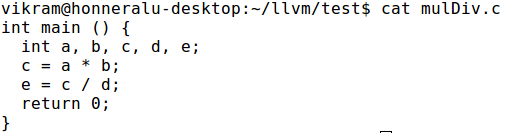
\includegraphics[scale=0.50]{./mulDiv.png}
\else
\fi
\caption[A simple test case]{A simple example}
\label{fig:ex1}
\end{center}
\end{figure}

\begin{figure}[!h]
\begin{center}
\ifpdf
	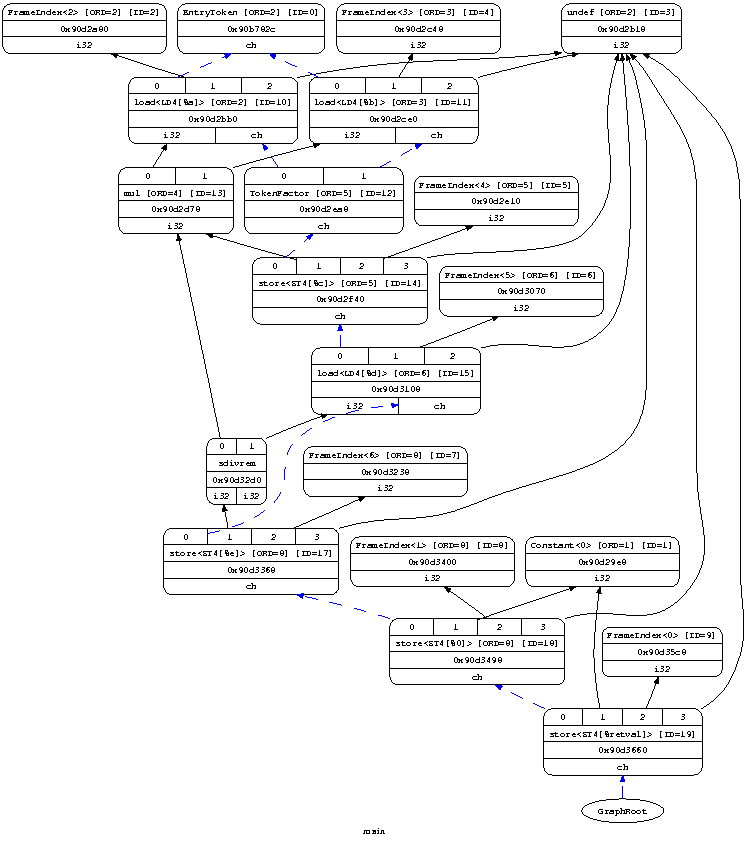
\includegraphics[scale=0.50, totalheight=0.62\textheight  ]{./mulDivDAG.png}
\else
\fi
\caption{MRIS DAG}
\label{fig:DAG}
\end{center}
\end{figure}

The set of lineages formed are as shown in figure \ref{fig:lineages}. The corresponding reach matrix is as shown in figure \ref{fig:reachmat}. After fusions, the reach matrix will be as shown in figure \ref{fig:fusion} and the lineages will be as shown in figure \ref{fig:lineagesfusion}. Finally, the sequence generated using lineages will be as shown in figure \ref{fig:finalseq}. This program had an HRB of 2.

\clearpage

\begin{figure}[!h]
\begin{center}
\ifpdf
	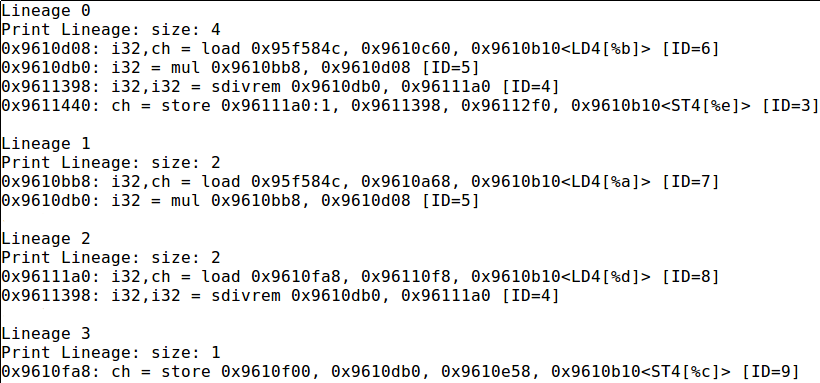
\includegraphics[scale=0.50]{./lineageFormation.png}
\else
\fi
\caption{Lineages formed}
\label{fig:lineages}
\end{center}
\end{figure}

\begin{figure}[!h]
\begin{center}
\ifpdf
	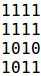
\includegraphics[scale=.5]{./reachMatrix.png}
\else
\fi
\caption{Reach Matrix}
\label{fig:reachmat}
\end{center}
\end{figure}

\begin{figure}[!h]
\begin{center}
\ifpdf
	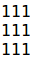
\includegraphics[scale=.5]{./reachMatrixAfterFusion.png}
\else
\fi
\caption{Reach Matrix after fusions}
\label{fig:fusion}
\end{center}
\end{figure}

\begin{figure}[!h]
\begin{center}
\ifpdf
	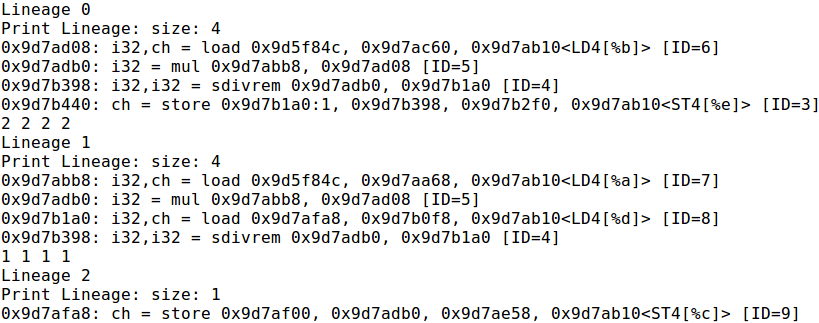
\includegraphics[scale=0.50]{./lineagesAfterFusion.png}
\else
\fi
\caption{Lineages after fusions}
\label{fig:lineagesfusion}
\end{center}
\end{figure}

\begin{figure}[!h]
\begin{center}
\ifpdf
	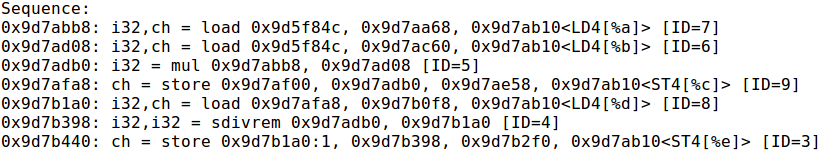
\includegraphics[scale=0.50]{./finalSequence.png}
\else
\fi
\caption{Final Sequence}
\label{fig:finalseq}
\end{center}
\end{figure}

Consider another program code as shown in figure \ref{fig:ex2}. The sequence generated for this program is shown in figure \ref{fig:seq} and had an HRB of 3.

\begin{figure}[!h]
\begin{center}
\ifpdf
	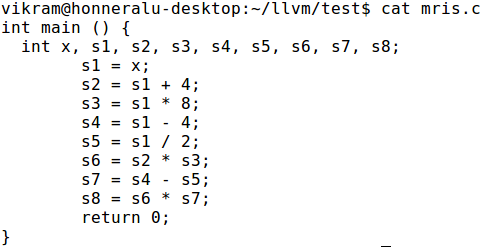
\includegraphics[scale=0.50]{./mrisCode.png}
\else
\fi
\caption{MRIS example code}
\label{fig:ex2}
\end{center}
\end{figure}

\begin{figure}[!h]
\begin{center}
\ifpdf
	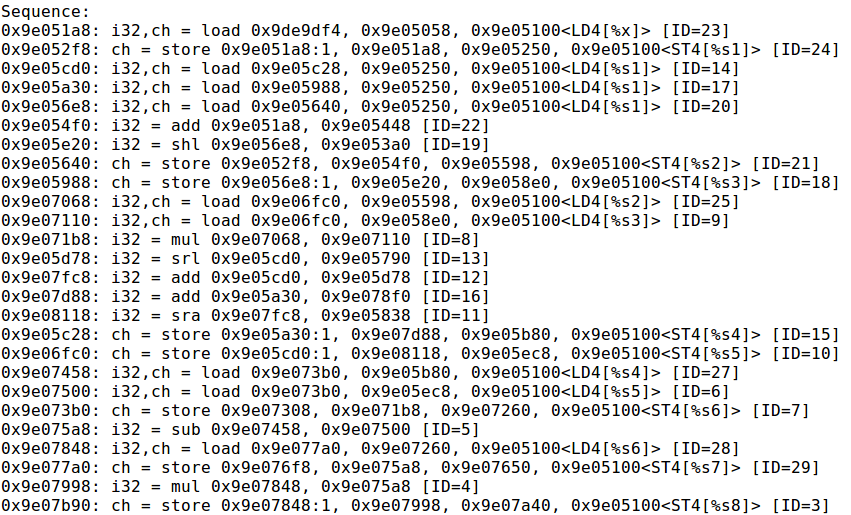
\includegraphics[scale=0.45]{./mrisSequence.png}
\else
\fi
\caption{Sequence for MRIS example code}
\label{fig:seq}
\end{center}
\end{figure}

\section{Example 2 - if-else Operation}

Consider another example involving an if-else construct. The code is shown in the figure \ref{fig:if-else}. Figures \ref{fig:BB1} - \ref{fig:LBB5}  show the data-dependency graphs generated for the basic blocks of the if-else construct, their corresponding lineages after lineage fusions and the final sequence.\\

\begin{figure}[!h]
\begin{center}
\ifpdf
	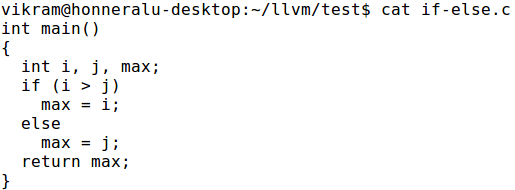
\includegraphics[scale=0.50]{./if-else-images/if-else.png}
\else
\fi
\caption{if-else Structure}
\label{fig:if-else}
\end{center}
\end{figure}

\begin{figure}[!h]
\begin{center}
\ifpdf
	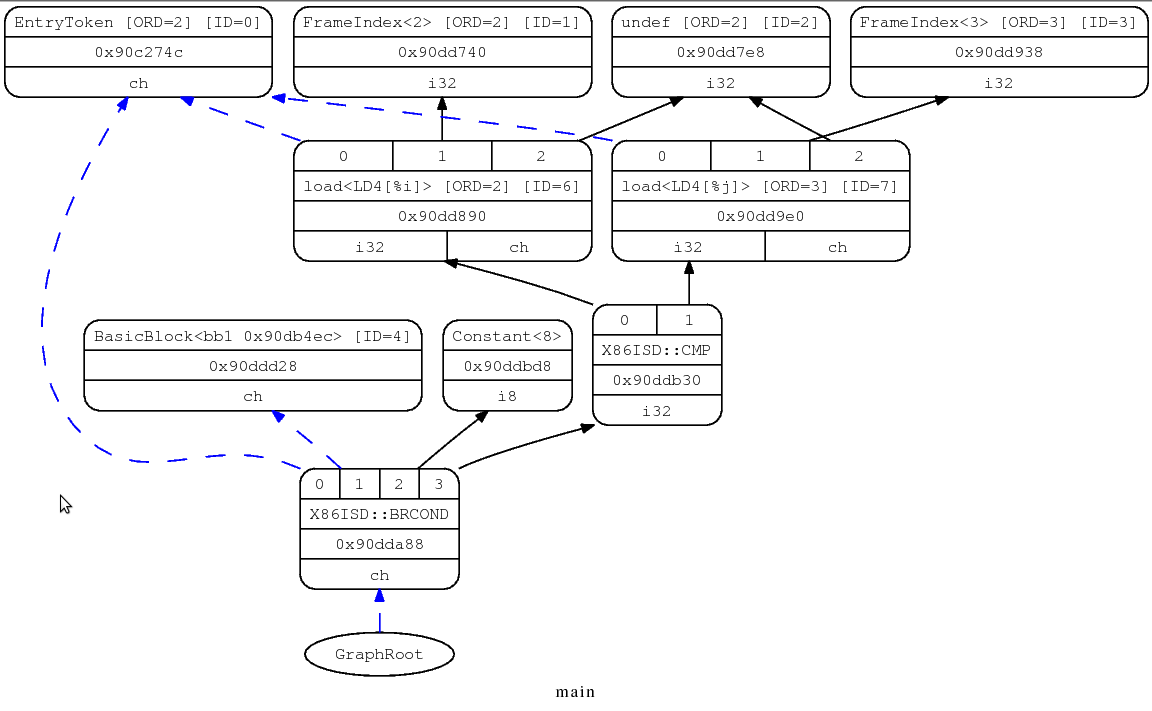
\includegraphics[scale=0.30]{./if-else-images/bb1.png}
\else
\fi
\caption{BB1 for if-else}
\label{fig:BB1}
\end{center}
\end{figure}

\begin{figure}[h]
\begin{center}
\ifpdf
	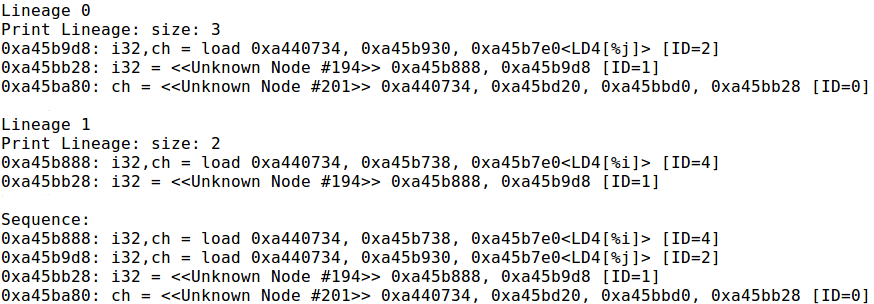
\includegraphics[scale=0.45]{./if-else-images/bbLineageSeq1.png}
\else
\fi
\caption{Lineages and final sequence for BB1 of if-else}
\label{fig:LBB1}
\end{center}
\end{figure}

\begin{figure}[h]
\begin{center}
\ifpdf
	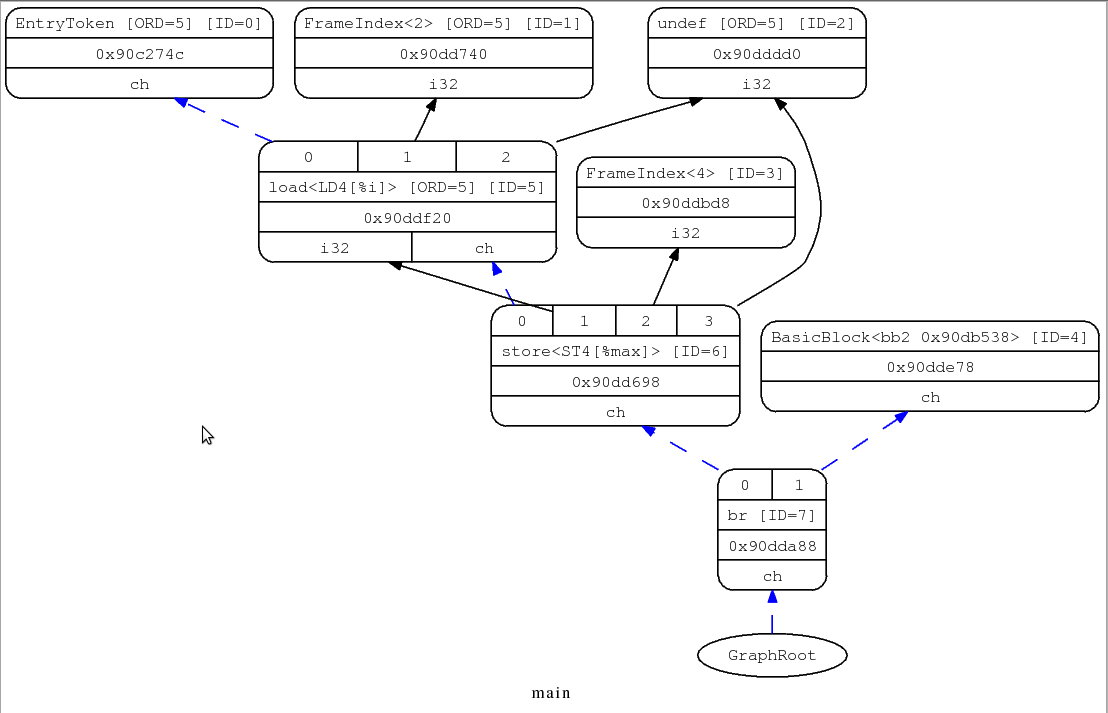
\includegraphics[scale=0.30]{./if-else-images/bb2.png}
\else
\fi
\caption{BB2 for if-else}
\label{fig:BB2}
\end{center}
\end{figure}

\begin{figure}[h]
\begin{center}
\ifpdf
	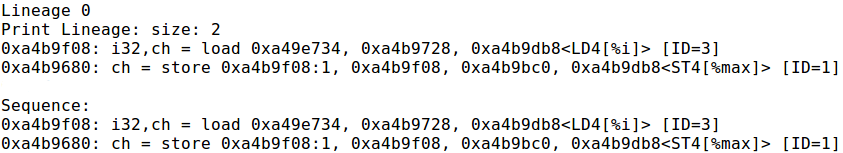
\includegraphics[scale=0.50]{./if-else-images/bbLineageSeq2.png}
\else
\fi
\caption{Lineages and final sequence for BB2 of if-else}
\label{fig:LBB2}
\end{center}
\end{figure}

\begin{figure}[h]
\begin{center}
\ifpdf
	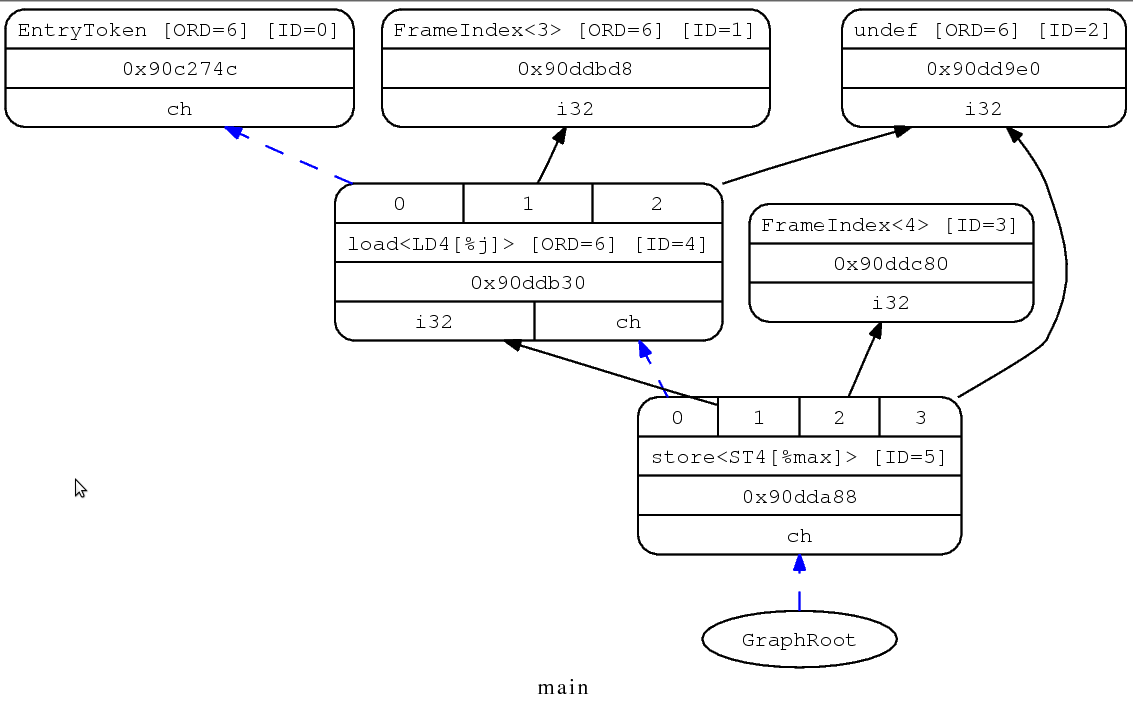
\includegraphics[scale=0.30]{./if-else-images/bb3.png}
\else
\fi
\caption{BB3 for if-else}
\label{fig:BB3}
\end{center}
\end{figure}

\begin{figure}[h]
\begin{center}
\ifpdf
	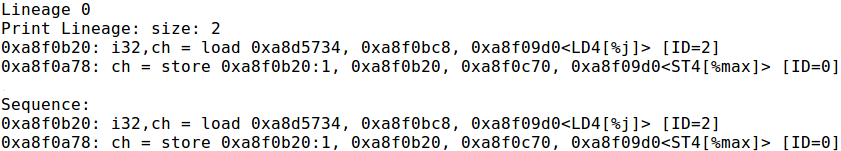
\includegraphics[scale=0.50]{./if-else-images/bbLineageSeq3.png}
\else
\fi
\caption{Lineages and final sequence for BB3 of if-else}
\label{fig:LBB3}
\end{center}
\end{figure}

\begin{figure}[h]
\begin{center}
\ifpdf
	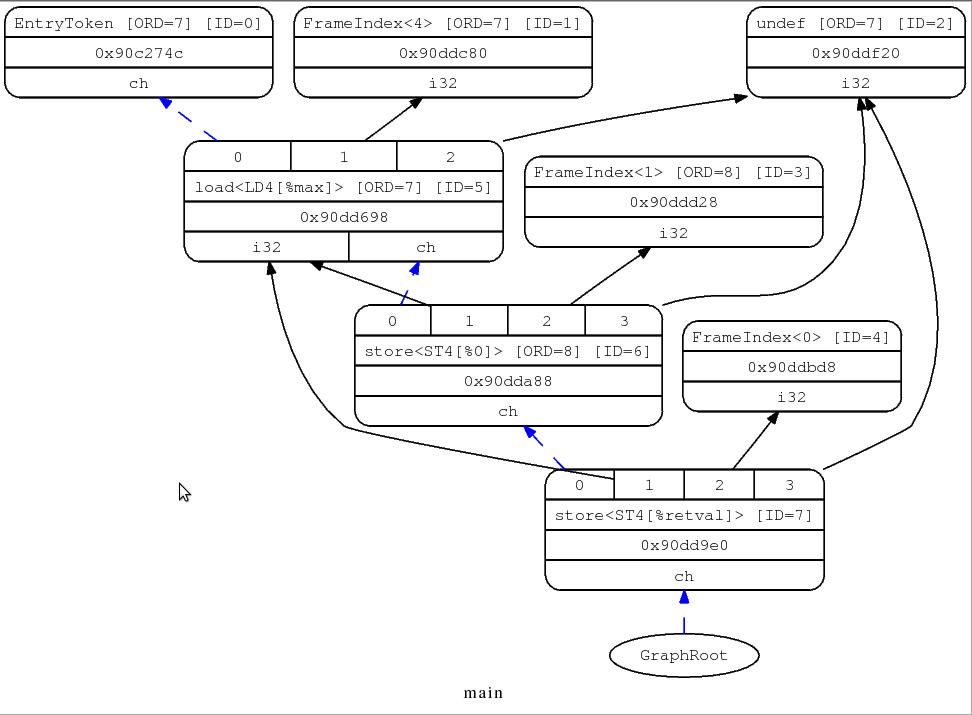
\includegraphics[scale=0.30]{./if-else-images/bb4.png}
\else
\fi
\caption{BB4 for if-else}
\label{fig:BB4}
\end{center}
\end{figure}

\begin{figure}[h]
\begin{center}
\ifpdf
	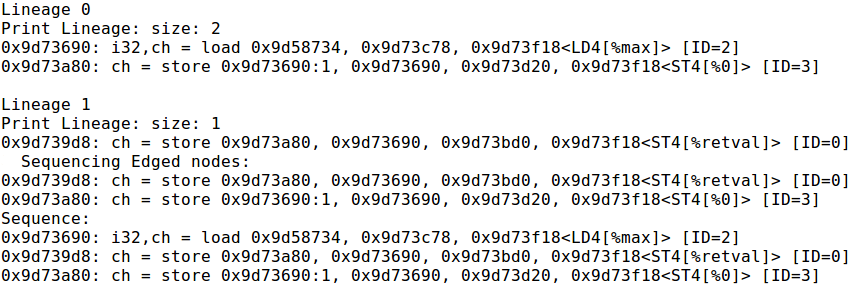
\includegraphics[scale=0.50]{./if-else-images/bbLineageSeq4.png}
\else
\fi
\caption{Lineages and final sequence for BB4 of if-else}
\label{fig:LBB4}
\end{center}
\end{figure}

\begin{figure}[h]
\begin{center}
\ifpdf
	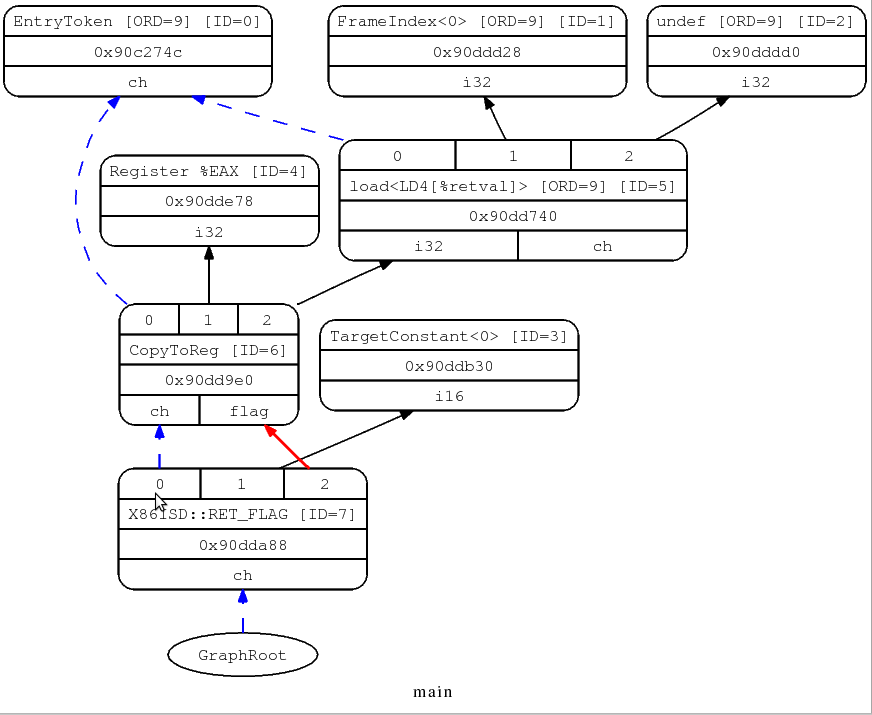
\includegraphics[scale=0.30]{./if-else-images/bb5.png}
\else
\fi
\caption{BB5 for if-else: \emph{max} gets returned}
\label{fig:BB5}
\end{center}
\end{figure}

\begin{figure}[h]
\begin{center}
\ifpdf
	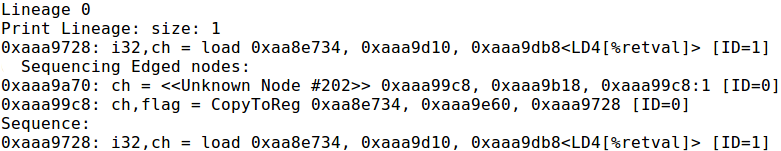
\includegraphics[scale=0.50]{./if-else-images/bbLineageSeq5.png}
\else
\fi
\caption{Lineages and final sequence for BB5 of if-else}
\label{fig:LBB5}
\end{center}
\end{figure}


\chapter{Conclusions and Future Work}

In this project we try to improve on the traditional instruction scheduling problem by implementing the MRIS approach. In traditional instruction scheduling, the emphasis on reducing the execution time of the program. The scheduler takes into account the execution latencies of different instructions and availability of functional units, and then schedules a sequence which gives a minimum execution time. Here the scheduler does not optimize the number of register used in the execution. The scheduler tries to minimize the code length (schedule length) using a fixed number of registers. In contrast the MRIS approach emphasises on reducing the number of registers used. The MRIS problem is closely related to \emph{optimal code generation} problem.\\

MRIS approach uses heuristic approach by calculating lineages, interference graph and uses an efficient list scheduling algorithm to find a near optimum solution for the problem. The register allocator then allocates available registers to each of the lineages. The coloring algorithm estimates HRB number of registers and in most of the cases with the number of registers actually used is less than or equal to the HRB value predicted. In some cases where it is impossible to allocate registers using only the HRB number, we increment the number of registers by one until a legal instruction sequence is generated with as little extra registers used.\\

The traditional instruction scheduler does not try to minimize the register pressure and hence the register allocator has to spill instructions when the register pressure increases beyond the total number of available register. The spilled instructions will hinder the performance and execution time of the program. MRIS approach minimizes the number of spills thus improving the execution time. MRIS approach might also allow a smaller cache and reduce the traffic of data between the processor and the main memory. We like to evaluate the performance of our heuristic approach of MRIS problem on various benchmarks. The experimental study and evaluating the performance leaves the scope for future work.

\singlespacing

\begin{thebibliography}{50}
\bibitem{Aho} A.V. Aho, R. Sethi, and J.D. Ullman, \emph{"Compilers - Principles, Techniques, and Tools"}, corrected ed. Reading, Mass.: Addison-Wesley, 1988.
\bibitem{Ullman} A.V. Aho, J.E. Hopcroft, J.D. Ullman: The Design and Analysis of Computer Algorithms. Addison-Wesley, 1974.
\bibitem{Appel} Andrew W. Appel, \emph{"Modern Compiler Implementation in C"}, Revised Edition, Cambridge University Press, 2000.
\bibitem{Briggs} P. Briggs, K.D. Cooper, and L. Torczon, \emph{"Improvements to Graph Coloring Register Allocation"}, \emph{ACM Trans. Programming Languages and Systems}, May 1994.
\bibitem{Chaitin} G.J. Chaitin, \emph{"Register Allocation and Spilling via Graph Coloring"}, Proc. \emph{SIGPLAN '82 Symp. Compiler Construction}, June 1982.
\bibitem{Cormen} T.H. Cormen, C.E. Leiserson, R.L. Rivest, C. Stein: Introduction to Algorithms. 2nd edition, The MIT Press, 2001.
\bibitem{Gibbons-Muchnick} P.B. Gibbons and S.S. Muchnick, \emph{"Efficient Instruction Scheduling for a Pipelined Architecture"}, \emph{Proc. SIGPLAN '86 Symp. Compiler Construction}, June 1986.
\bibitem{R. Govindarajan et al.} R. Govindarajan, H. Yang, J.N. Amaral, C. Zhang, and G.R. Gao, \emph{"Minimum Register Instruction Sequencing to Reduce Register Spills in Out-Of-Order Issue Superscalar Architectures"}, IEEE Transactions on Computers, Vol. 52, No. 1, January 2003.
\bibitem{Lamport}  Leslie Lamport,  \emph{\LaTeX: A Document Preparation System}.  Addison-Wesley, Massachusetts,  2nd Edition,  1994.
\bibitem{Primer} S.B. Lippman, and J. Lajoie, \emph{"C++ Primer"}, Third Edition, Addison-Wesley, March 1998.
\bibitem{Muchnick} S.S. Muchnick, \emph{"Advanced Compiler Design and Implementation"}. San Francisco: Morgan Kaufmann, 1997.
\bibitem{Architecture} D.A. Patterson, and J.L. Hennessy, \emph{"Computer Architecture : A Quantitative Approach"}, Reading, Morgan Kaufmann, 4th ed., 2007
\bibitem{Hennessy-Patterson} D.A. Patterson, and J.L. Hennessy, \emph{"Computer Organization and Design: The Hardware/Software Interface"}, Second Edition, Harcourt Asia, Morgan Kaufmann, 1998.
\bibitem{Poletto-Sarkar} M. Poletto and V. Sarkar, \emph{"Linear Scan Register Allocation"}, \emph{ACM Trans. Programming Languages and Systems}, 1998.
\bibitem{C++ Reference} H. Schildt, \emph{"C++ : The Complete Reference"}, Third Edition, Osborne McGraw-Hill.
\bibitem{LLVM} Source code \href{http://llvm.org/}{http://llvm.org/}
\end{thebibliography}
\fancyfoot[LO,LE]{This document was produced by \LaTeX.}

\end{document}
